\documentclass{standalone}
\usepackage{tikz}
\usetikzlibrary{patterns, positioning}
\usepackage[sfdefault]{ClearSans} %% option 'sfdefault' activates Clear Sans as the default text font
\usepackage[T1]{fontenc}

\begin{document}
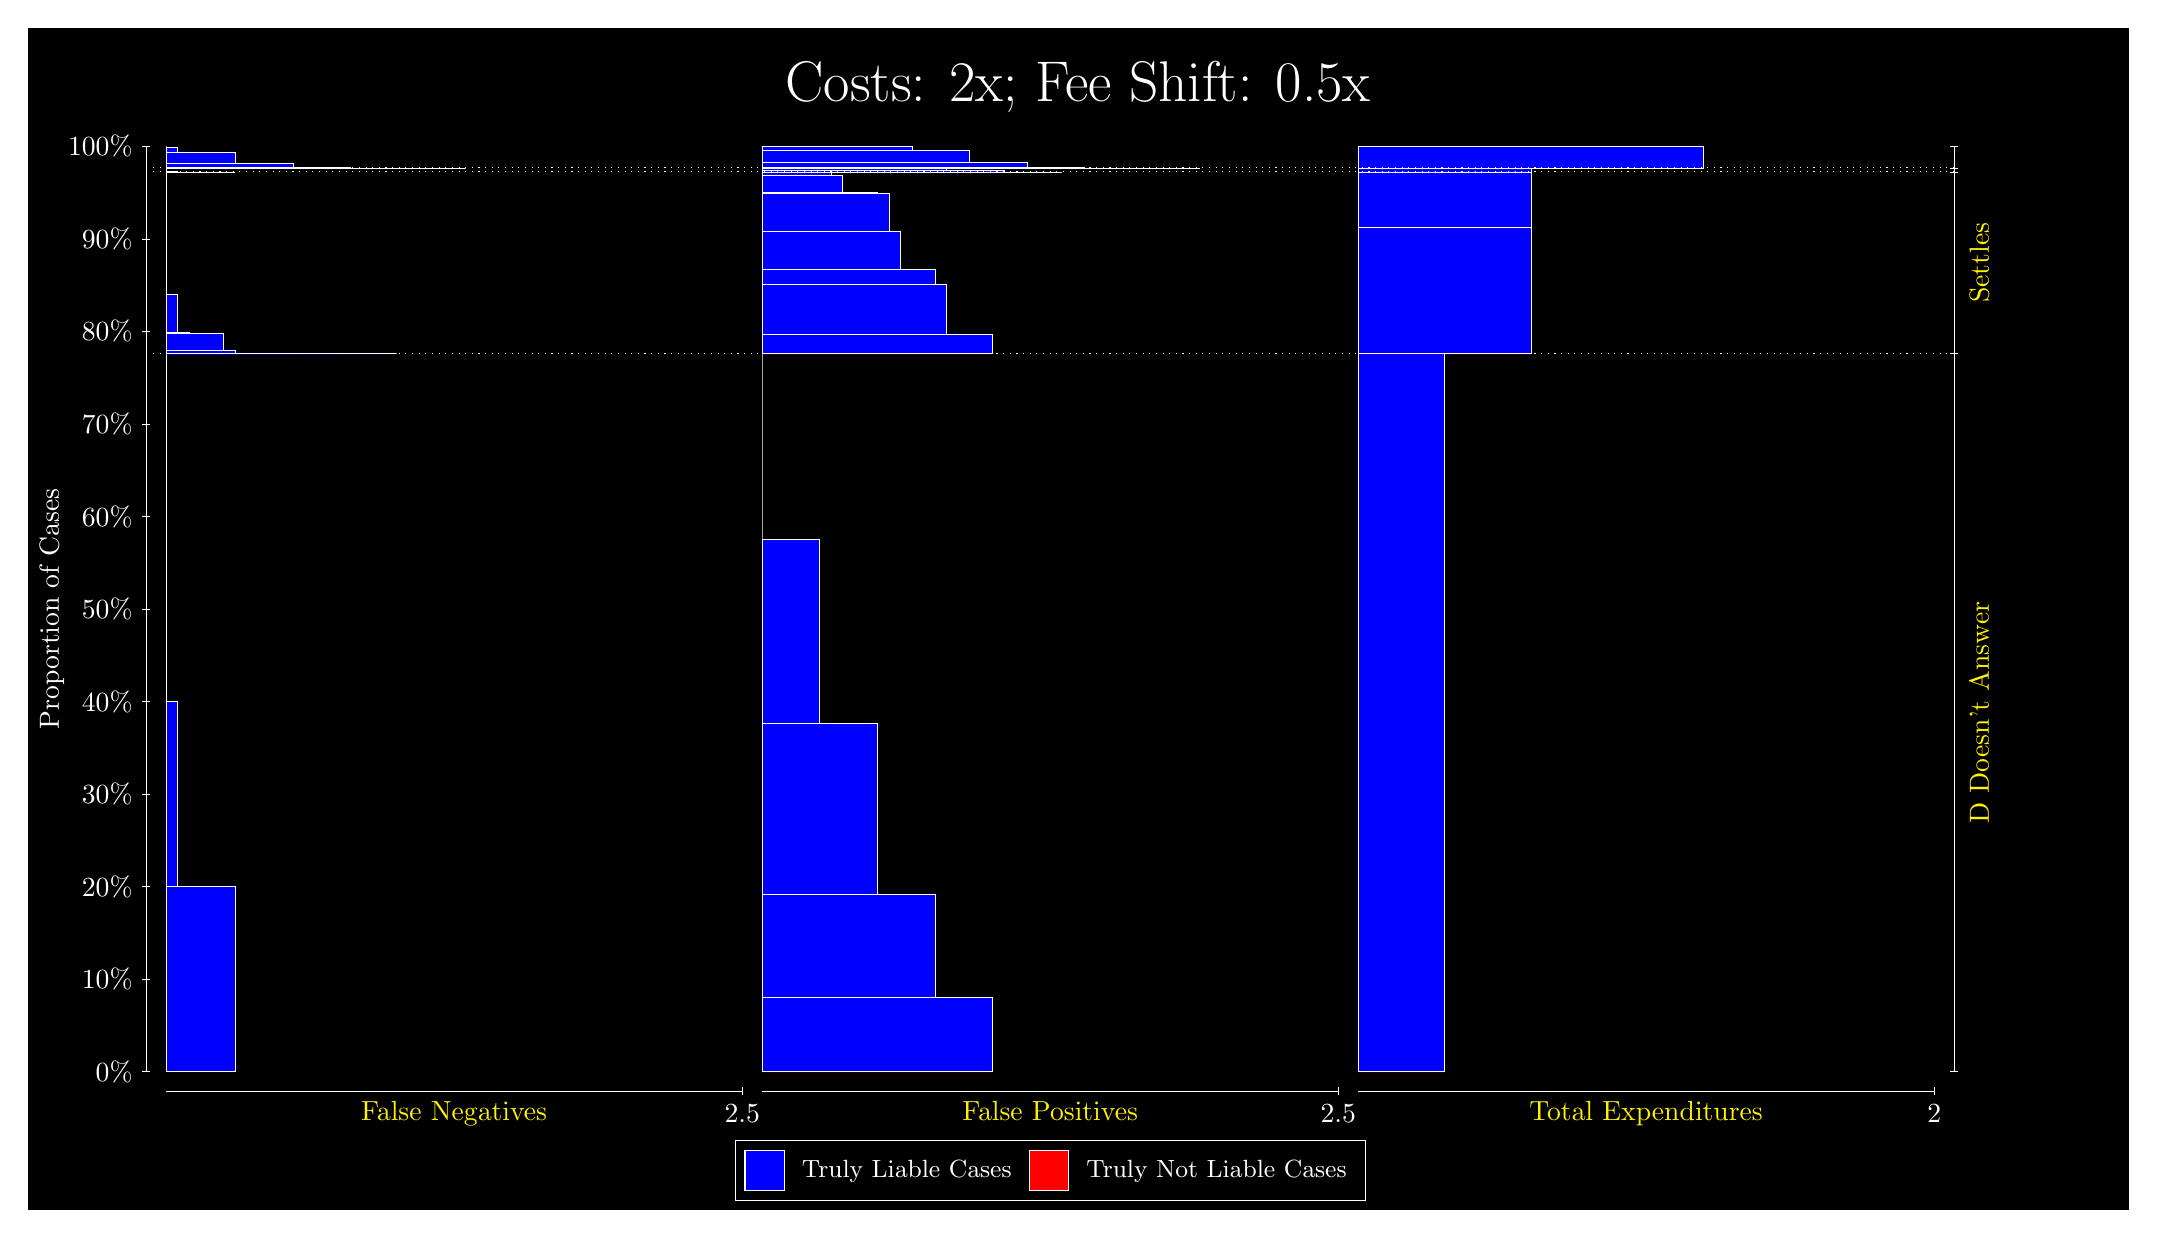
\begin{tikzpicture}
\draw[fill=black] (0,0) rectangle (26.667,15);
\draw[text=white] (0,13.5) rectangle (26.667,15) node[midway] {\huge Costs: 2x; Fee Shift: 0.5x};
\draw[white, very thin] (1.5,1.75) -- (1.5,13.5);
\node[rotate=90, text=white, anchor=center] at (0.3, 7.625) {Proportion of Cases};
\draw[white, very thin] (1.45,1.75) -- (1.55,1.75);
\node[text=white, anchor=east] at (1.45, 1.75) {0\%};
\draw[white, very thin] (1.45,2.925) -- (1.55,2.925);
\node[text=white, anchor=east] at (1.45, 2.925) {10\%};
\draw[white, very thin] (1.45,4.1) -- (1.55,4.1);
\node[text=white, anchor=east] at (1.45, 4.1) {20\%};
\draw[white, very thin] (1.45,5.275) -- (1.55,5.275);
\node[text=white, anchor=east] at (1.45, 5.275) {30\%};
\draw[white, very thin] (1.45,6.45) -- (1.55,6.45);
\node[text=white, anchor=east] at (1.45, 6.45) {40\%};
\draw[white, very thin] (1.45,7.625) -- (1.55,7.625);
\node[text=white, anchor=east] at (1.45, 7.625) {50\%};
\draw[white, very thin] (1.45,8.8) -- (1.55,8.8);
\node[text=white, anchor=east] at (1.45, 8.8) {60\%};
\draw[white, very thin] (1.45,9.975) -- (1.55,9.975);
\node[text=white, anchor=east] at (1.45, 9.975) {70\%};
\draw[white, very thin] (1.45,11.15) -- (1.55,11.15);
\node[text=white, anchor=east] at (1.45, 11.15) {80\%};
\draw[white, very thin] (1.45,12.325) -- (1.55,12.325);
\node[text=white, anchor=east] at (1.45, 12.325) {90\%};
\draw[white, very thin] (1.45,13.5) -- (1.55,13.5);
\node[text=white, anchor=east] at (1.45, 13.5) {100\%};

\draw[white, very thin] (24.457,1.75) -- (24.457,13.5);
\draw[white, very thin] (24.407,1.75) -- (24.507,1.75);
\node[anchor=west] at (24.407, 1.75) {};
\draw[white, very thin] (24.407,10.866) -- (24.507,10.866);
\node[anchor=west] at (24.407, 10.866) {};
\draw[white, very thin] (24.407,13.176) -- (24.507,13.176);
\node[anchor=west] at (24.407, 13.176) {};
\draw[white, very thin] (24.407,13.226) -- (24.507,13.226);
\node[anchor=west] at (24.407, 13.226) {};
\draw[white, very thin] (24.407,13.5) -- (24.507,13.5);
\node[anchor=west] at (24.407, 13.5) {};

\draw[white, very thin, fill=blue] (1.75,1.75) rectangle (2.6283,4.0999);
\draw[white, very thin, fill=blue] (1.75,4.0999) rectangle (1.8964,6.4484);
\draw[white, very thin, fill=red] (1.75,6.4484) rectangle (1.75,6.4484);
\draw[white, very thin, fill=blue] (1.75,6.4484) rectangle (1.75,10.866);
\draw[white, very thin, fill=blue] (1.75,10.866) rectangle (4.6775,10.866);
\draw[white, very thin, fill=blue] (1.75,10.866) rectangle (4.092,10.866);
\draw[white, very thin, fill=blue] (1.75,10.866) rectangle (3.9457,10.866);
\draw[white, very thin, fill=blue] (1.75,10.866) rectangle (3.5065,10.866);
\draw[white, very thin, fill=blue] (1.75,10.866) rectangle (3.3602,10.866);
\draw[white, very thin, fill=blue] (1.75,10.866) rectangle (3.2138,10.873);
\draw[white, very thin, fill=blue] (1.75,10.873) rectangle (2.7746,10.873);
\draw[white, very thin, fill=blue] (1.75,10.873) rectangle (2.6283,10.909);
\draw[white, very thin, fill=blue] (1.75,10.909) rectangle (2.4819,11.125);
\draw[white, very thin, fill=blue] (1.75,11.125) rectangle (2.0428,11.143);
\draw[white, very thin, fill=blue] (1.75,11.143) rectangle (1.8964,11.617);
\draw[white, very thin, fill=red] (1.75,11.617) rectangle (1.75,11.617);
\draw[white, very thin, fill=blue] (1.75,11.617) rectangle (1.75,13.176);
\draw[white, very thin, fill=blue] (1.75,13.176) rectangle (2.6283,13.176);
\draw[white, very thin, fill=blue] (1.75,13.176) rectangle (1.8964,13.177);
\draw[white, very thin, fill=red] (1.75,13.177) rectangle (1.75,13.177);
\draw[white, very thin, fill=blue] (1.75,13.177) rectangle (1.75,13.226);
\draw[white, very thin, fill=blue] (1.75,13.226) rectangle (5.5558,13.226);
\draw[white, very thin, fill=blue] (1.75,13.226) rectangle (4.8239,13.226);
\draw[white, very thin, fill=blue] (1.75,13.226) rectangle (4.092,13.228);
\draw[white, very thin, fill=blue] (1.75,13.228) rectangle (3.3602,13.281);
\draw[white, very thin, fill=blue] (1.75,13.281) rectangle (2.6283,13.281);
\draw[white, very thin, fill=blue] (1.75,13.281) rectangle (2.6283,13.426);
\draw[white, very thin, fill=blue] (1.75,13.426) rectangle (1.8964,13.426);
\draw[white, very thin, fill=blue] (1.75,13.426) rectangle (1.8964,13.493);
\draw[white, very thin, fill=red] (1.75,13.493) rectangle (1.75,13.493);
\draw[white, very thin, fill=blue] (1.75,13.493) rectangle (1.75,13.5);
\draw[white, very thin, fill=red] (9.3189,1.75) rectangle (12.246,1.75);
\draw[white, very thin, fill=blue] (9.3189,1.75) rectangle (12.246,2.6885);
\draw[white, very thin, fill=blue] (9.3189,2.6885) rectangle (11.515,4.0039);
\draw[white, very thin, fill=blue] (9.3189,4.0039) rectangle (10.783,6.1672);
\draw[white, very thin, fill=blue] (9.3189,6.1672) rectangle (10.051,8.5156);
\draw[white, very thin, fill=blue] (9.3189,8.5156) rectangle (9.3189,10.866);
\draw[white, very thin, fill=red] (9.3189,10.866) rectangle (12.246,10.866);
\draw[white, very thin, fill=blue] (9.3189,10.866) rectangle (12.246,11.114);
\draw[white, very thin, fill=red] (9.3189,11.114) rectangle (11.661,11.114);
\draw[white, very thin, fill=blue] (9.3189,11.114) rectangle (11.661,11.745);
\draw[white, very thin, fill=blue] (9.3189,11.745) rectangle (11.515,11.939);
\draw[white, very thin, fill=red] (9.3189,11.939) rectangle (11.075,11.939);
\draw[white, very thin, fill=blue] (9.3189,11.939) rectangle (11.075,12.425);
\draw[white, very thin, fill=blue] (9.3189,12.425) rectangle (10.929,12.899);
\draw[white, very thin, fill=blue] (9.3189,12.899) rectangle (10.783,12.917);
\draw[white, very thin, fill=blue] (9.3189,12.917) rectangle (10.344,13.132);
\draw[white, very thin, fill=blue] (9.3189,13.132) rectangle (10.197,13.169);
\draw[white, very thin, fill=blue] (9.3189,13.169) rectangle (10.051,13.169);
\draw[white, very thin, fill=blue] (9.3189,13.169) rectangle (9.6116,13.176);
\draw[white, very thin, fill=blue] (9.3189,13.176) rectangle (9.4652,13.176);
\draw[white, very thin, fill=blue] (9.3189,13.176) rectangle (9.3189,13.176);
\draw[white, very thin, fill=red] (9.3189,13.176) rectangle (13.125,13.176);
\draw[white, very thin, fill=blue] (9.3189,13.176) rectangle (13.125,13.176);
\draw[white, very thin, fill=blue] (9.3189,13.176) rectangle (12.393,13.197);
\draw[white, very thin, fill=blue] (9.3189,13.197) rectangle (11.661,13.226);
\draw[white, very thin, fill=blue] (9.3189,13.226) rectangle (10.929,13.226);
\draw[white, very thin, fill=blue] (9.3189,13.226) rectangle (10.197,13.226);
\draw[white, very thin, fill=red] (9.3189,13.226) rectangle (14.881,13.226);
\draw[white, very thin, fill=blue] (9.3189,13.226) rectangle (14.881,13.226);
\draw[white, very thin, fill=red] (9.3189,13.226) rectangle (14.149,13.226);
\draw[white, very thin, fill=blue] (9.3189,13.226) rectangle (14.149,13.226);
\draw[white, very thin, fill=red] (9.3189,13.226) rectangle (13.417,13.226);
\draw[white, very thin, fill=blue] (9.3189,13.226) rectangle (13.417,13.233);
\draw[white, very thin, fill=red] (9.3189,13.233) rectangle (12.686,13.233);
\draw[white, very thin, fill=blue] (9.3189,13.233) rectangle (12.686,13.3);
\draw[white, very thin, fill=red] (9.3189,13.3) rectangle (11.954,13.3);
\draw[white, very thin, fill=blue] (9.3189,13.3) rectangle (11.954,13.445);
\draw[white, very thin, fill=blue] (9.3189,13.445) rectangle (11.222,13.498);
\draw[white, very thin, fill=blue] (9.3189,13.498) rectangle (10.49,13.5);
\draw[white, very thin, fill=blue] (9.3189,13.5) rectangle (9.758,13.5);
\draw[white, very thin, fill=blue] (9.3189,13.5) rectangle (9.3189,13.5);
\draw[white, very thin, fill=red] (16.888,1.75) rectangle (17.986,1.75);
\draw[white, very thin, fill=blue] (16.888,1.75) rectangle (17.986,10.866);
\draw[white, very thin, fill=red] (16.888,10.866) rectangle (19.083,10.866);
\draw[white, very thin, fill=blue] (16.888,10.866) rectangle (19.083,12.468);
\draw[white, very thin, fill=red] (16.888,12.468) rectangle (19.083,12.468);
\draw[white, very thin, fill=blue] (16.888,12.468) rectangle (19.083,13.176);
\draw[white, very thin, fill=red] (16.888,13.176) rectangle (19.083,13.176);
\draw[white, very thin, fill=blue] (16.888,13.176) rectangle (19.083,13.226);
\draw[white, very thin, fill=red] (16.888,13.226) rectangle (21.279,13.226);
\draw[white, very thin, fill=blue] (16.888,13.226) rectangle (21.279,13.5);
\draw[white, dotted] (1.5,10.866) -- (24.457,10.866);
\draw[white, dotted] (1.5,13.176) -- (24.457,13.176);
\draw[white, dotted] (1.5,13.226) -- (24.457,13.226);
\draw[white, very thin] (1.75,1.5) -- (9.0689,1.5);
\node[text=yellow, anchor=north] at (5.4094, 1.5) {False Negatives};
\draw[white, very thin] (9.0689,1.45) -- (9.0689,1.55);
\node[text=white, anchor=north] at (9.0689, 1.45) {2.5};

\draw[white, very thin] (9.3189,1.5) -- (16.638,1.5);
\node[text=yellow, anchor=north] at (12.978, 1.5) {False Positives};
\draw[white, very thin] (16.638,1.45) -- (16.638,1.55);
\node[text=white, anchor=north] at (16.638, 1.45) {2.5};

\draw[white, very thin] (16.888,1.5) -- (24.207,1.5);
\node[text=yellow, anchor=north] at (20.547, 1.5) {Total Expenditures};
\draw[white, very thin] (24.207,1.45) -- (24.207,1.55);
\node[text=white, anchor=north] at (24.207, 1.45) {2};

\node[text=yellow, centered, rotate=90] at (24.777, 6.3078) {D Doesn't Answer};
\node[text=yellow, centered, rotate=90] at (24.777, 12.021) {Settles};



\draw (12.978300999999998,1.5) node[draw=none] (baseCoordinate) {};
\begin{scope}[align=center]
        \matrix[scale=0.5, draw=white, below=0.5cm of baseCoordinate, nodes={draw}, column sep=0.1cm]{
            \node[rectangle, draw, minimum width=0.5cm, minimum height=0.5cm, fill=blue] {}; &
            \node[draw=none, font=\small, text=white] (B) {Truly Liable Cases}; &
            \node[rectangle, draw, minimum width=0.5cm, minimum height=0.5cm, fill=red] {}; &
            \node[draw=none, font=\small, text=white] (B) {Truly Not Liable Cases}; \\
            };
\end{scope}

\end{tikzpicture}
\end{document}